\documentclass[25pt,a1paper,landscape]{tikzposter}

%% Tikzposter is highly customizable: please see
%% https://bitbucket.org/surmann/tikzposter/downloads/styleguide.pdf

%% Available themes: see also
%% https://bitbucket.org/surmann/tikzposter/downloads/themes.pdf
\usetheme{Default}
% \usetheme{Rays}
% \usetheme{Basic}
%\usetheme{Simple}
% \usetheme{Envelope}
% \usetheme{Wave}
% \usetheme{Board}
% \usetheme{Autumn}
% \usetheme{Desert}


%% Further changes to the title etc is possible
% \usetitlestyle{Default}
% \usetitlestyle{Basic}
% \usetitlestyle{Empty}
% \usetitlestyle{Filled}
% \usetitlestyle{Envelope}
% \usetitlestyle{Wave}
% \usetitlestyle{verticalShading}

\colorlet{backgroundcolor}{white}
\usepackage{fontspec}
\usepackage{graphicx}
\usepackage{pdfpages}
\usepackage{mychronology}
\setmainfont{FreeSerif}
\setsansfont{FreeSans}

\title{Benoit Nadeau-Dostie}
%\author{1994 - 2024}
%% Optional title graphic
\titlegraphic{
	
\includegraphics[height=4cm]{images/UdeS2.jpg},
	
\includegraphics[height=4cm]{images/LogicVisionLogo3.jpg},
	
\includegraphics[height=4cm]{images/MGC Logo2.jpg},
	
\includegraphics[height=4cm]{images/Siemens2.png}
}
%% Uncomment to switch off tikzposter footer
% \tikzposterlatexaffectionproofoff
\def \pdfwidth{50mm}
\def \pdfheight{70mm}
\def \pdfoptions{width=\pdfwidth}
\settitle{ \centering \vbox{
%		\@titlegraphic \\[\TP@titlegraphictotitledistance] \centering
		\color{titlefgcolor} {\bfseries \Huge \sc \@title \par}
}}
\def \blw{1}
\tikzset{%
	,chronevent/.style={fill=black,draw=none,opacity=0.5}
	,chronlabel/.style={opacity=1}
	,chrontickslabel/.style={chronlabel}
	,chroneventlabel/.style={chronlabel}
	,eventlabel/.style={chroneventlabel,anchor=south west,yshift=.2\unit,rotate=0}
	,flippedeventlabel/.style={chroneventlabel,anchor=north west,yshift=-.2\unit,rotate=0}
	,eventlabelbottom/.style={chroneventlabel,anchor=south west,yshift=-1cm,rotate=0}     % Bottom label
}

\begin{document}
	
	%\tikz[remember picture,overlay] \node[opacity=0.3,inner sep=0pt] at (current page.center){
\includegraphics[width=\paperwidth,height=\paperheight]{images/PP_CHIP.png}};
	
	\maketitle   
    \end
 
	
	\block[linewidth=\blw]{}{
 		\begin{chronology}[2]{1984}{2024}{\linewidth}
		\event[1984]{1986}{
\includegraphics[height=2cm]{images/UdeS2.jpg}}
		\event[1986]{1994}{
\includegraphics[height=2cm]{images/Nortel.jpg}}
		\event[1994]{2009}{
%			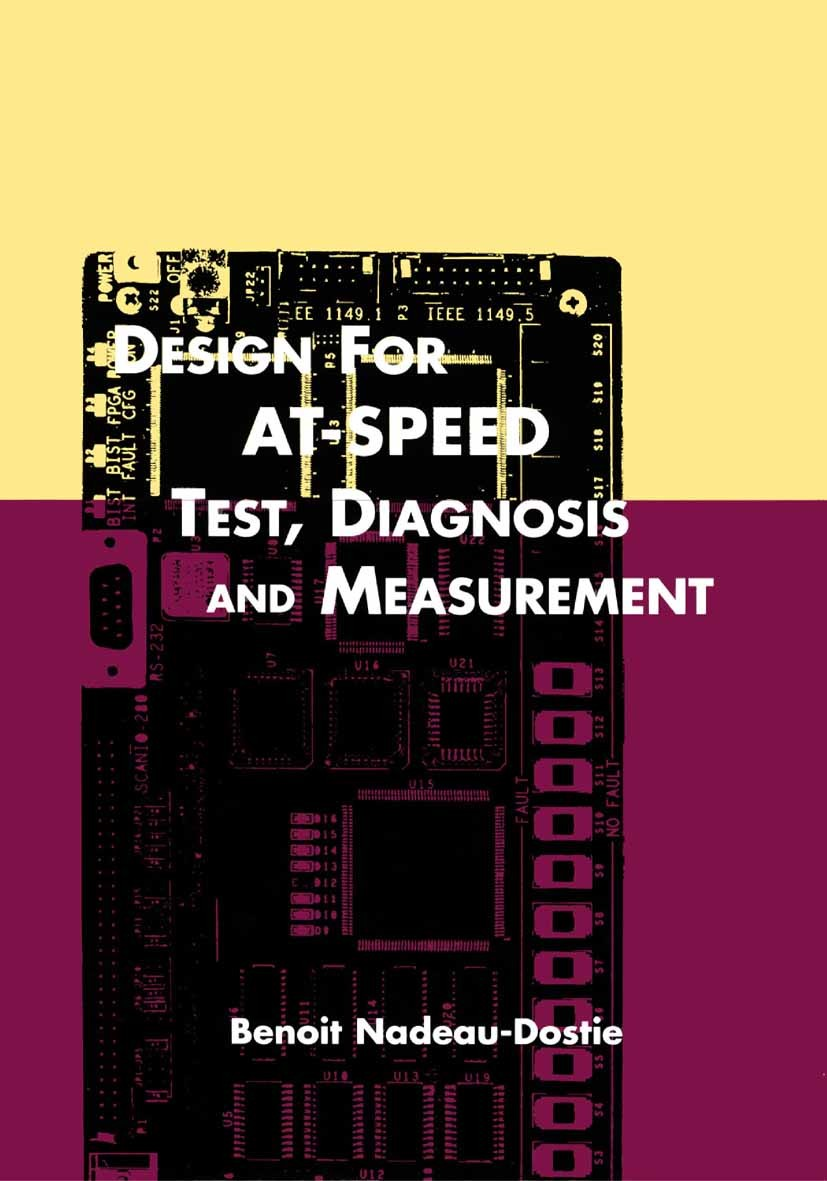
\includegraphics[height=4cm]{images/BND_Book.jpg}
			
\includegraphics[height=2cm]{images/LogicVisionLogo3.jpg},
			}
		\eventpoint{1999}{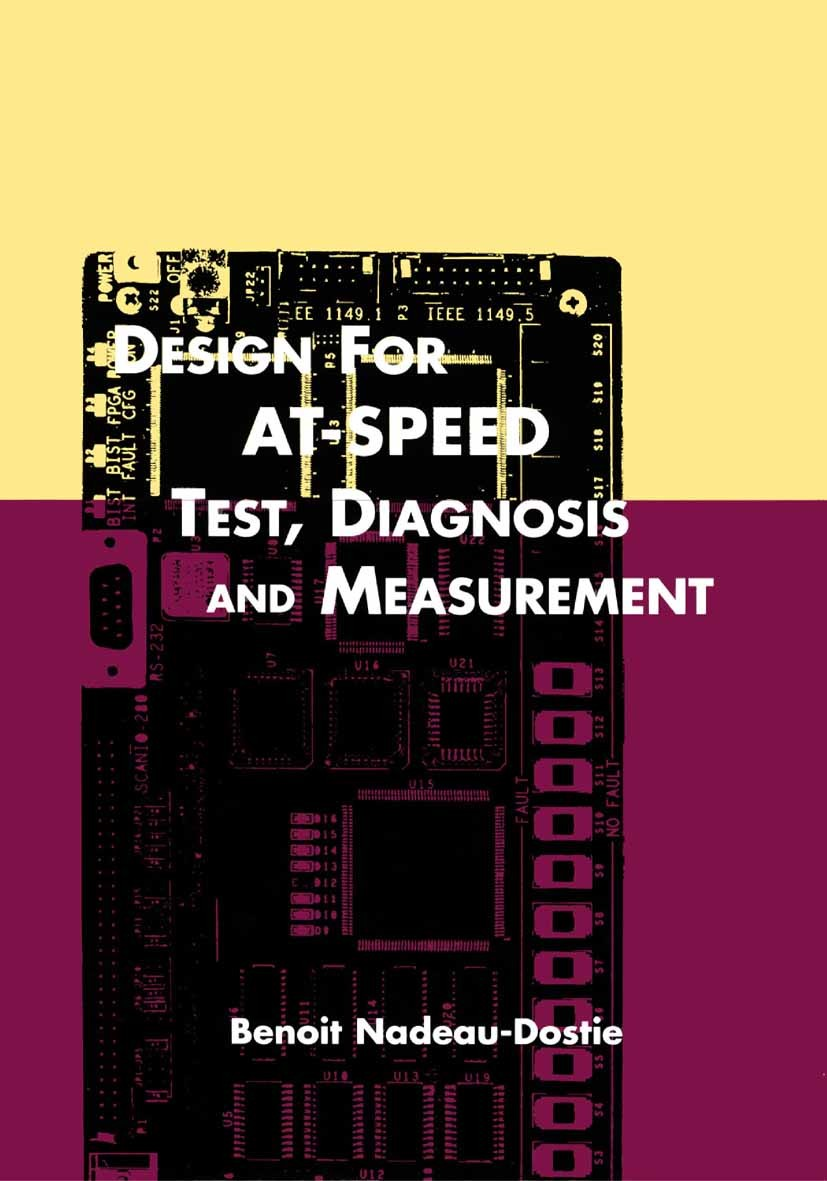
\includegraphics[height=4cm]{images/BND_Book.jpg}}
		\event[2009]{2017}{
\includegraphics[height=2cm]{images/MGC Logo2.jpg}}
		\event[2017]{2024}{
\includegraphics[height=2cm]{images/Siemens2.png}}
		\end{chronology}}
	
    %	\begin{tikzpicture}
	%	% draw horizontal line   
	%	\draw[ultra thick, ->] (0,0) -- (\linewidth,0);
	%	\foreach \x in {0,5,10,15,20,25,30,35,40,45,50,55,60,65,70,75}
	%	\draw (\x cm,3pt) -- (\x cm,-3pt);
	%	\draw[ultra thick] (5,0) node[below=3pt,thick] {1985} node[above=3pt] {};
	%	\draw[ultra thick] (10,0) node[below=3pt,thick] {1990} node[above=3pt] {};
	%	\draw[ultra thick] (15,0) node[below=3pt,thick] {1995} node[above=3pt] {};
	%	\draw[ultra thick] (20,0) node[below=3pt,thick] {2000} node[above=3pt] {};
	%	\draw[ultra thick] (25,0) node[below=3pt,thick] {2005} node[above=3pt] {};
	%	\draw[ultra thick] (30,0) node[below=3pt,thick] {2010} node[above=3pt] {};		
			
	%	\draw[fill=black,draw=none,opacity=0.5,rounded corners=10](10,-0.5) rectangle (20,0.5)%
	%	\draw (10,2) node{
\includegraphics[height=2cm]{images/UdeS2.jpg}}


	%	\end{tikzpicture}
	}
	

	\begin{columns}
		
		\column{0.5}
		\block[linewidth=\blw]{Publications}{
			\frame{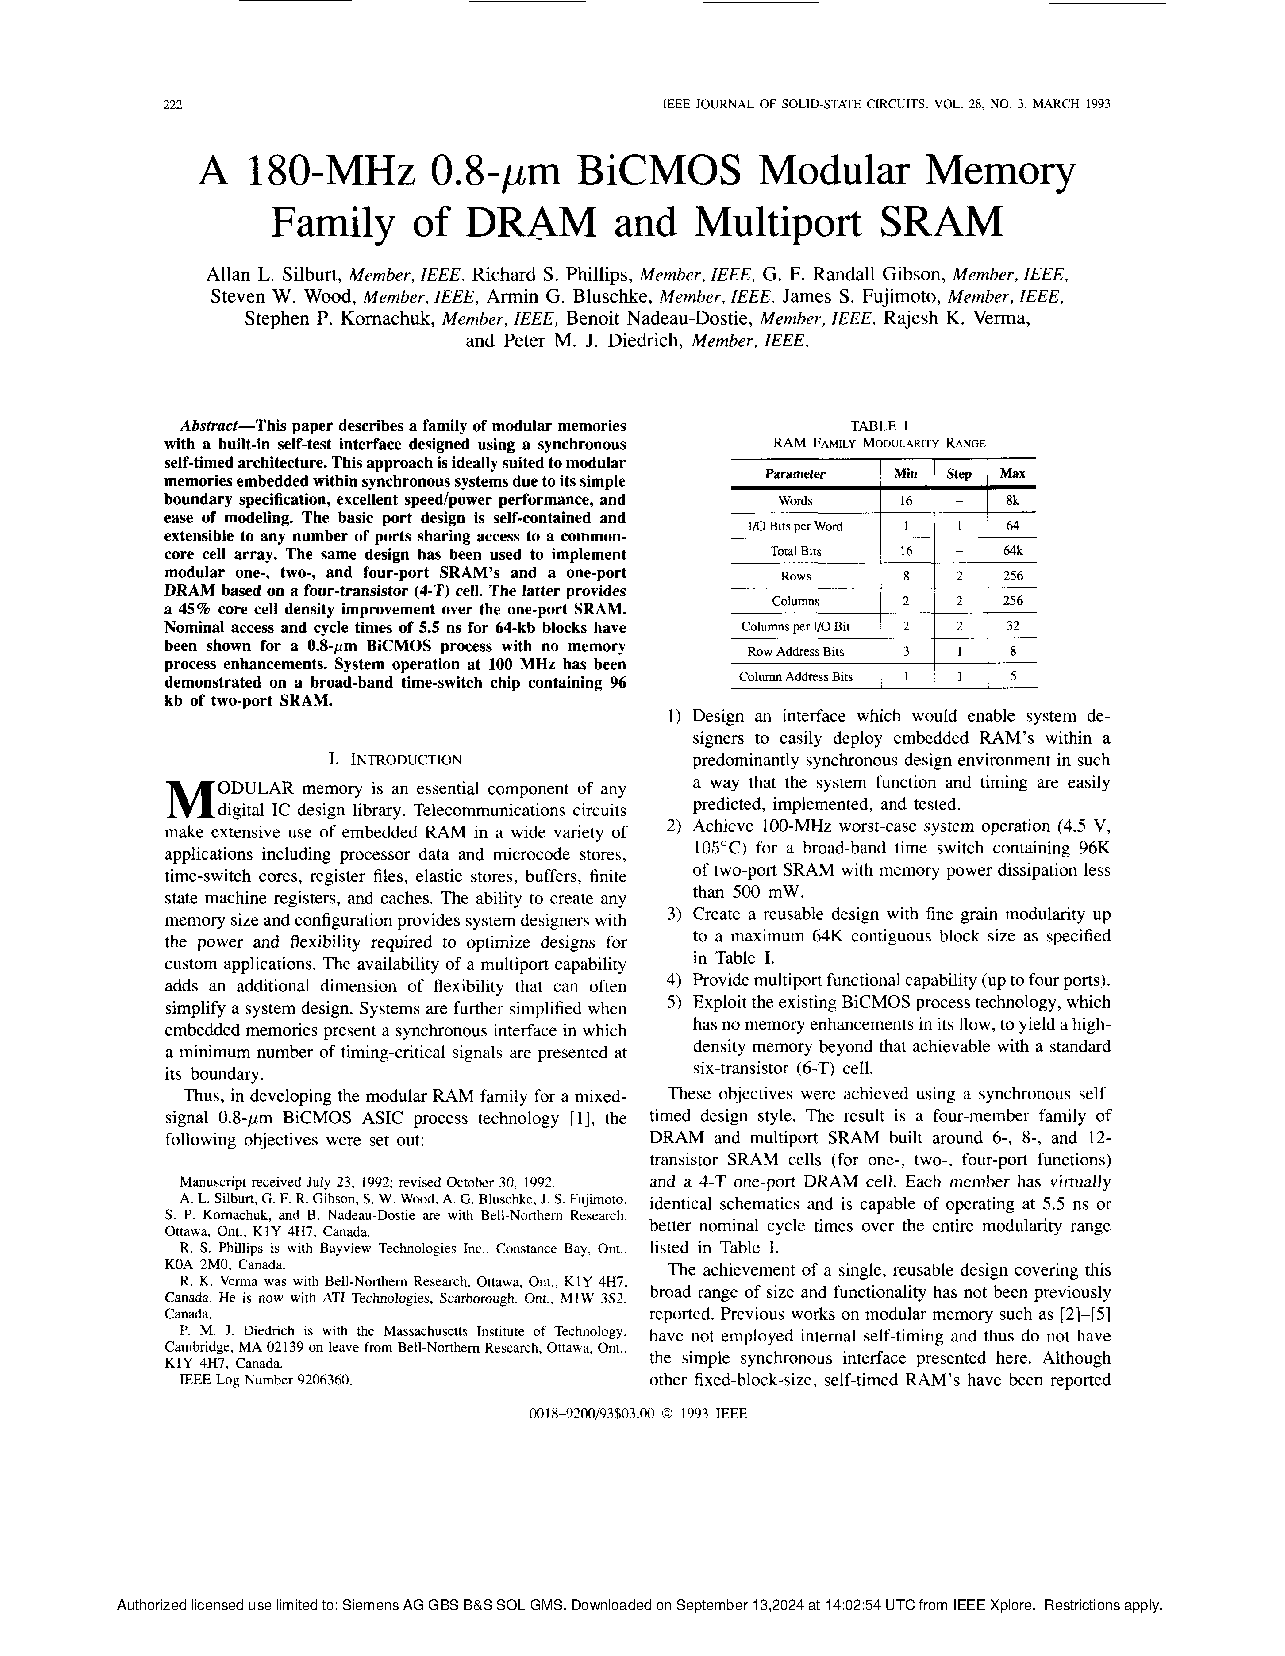
\includegraphics[height=\pdfheight]{Articles/publications/A_180_MHz_0.8_mu_m_BiCMOS_modular_memory_family_of_DRAM_and_multiport_SRAM-page1.pdf}}
			\frame{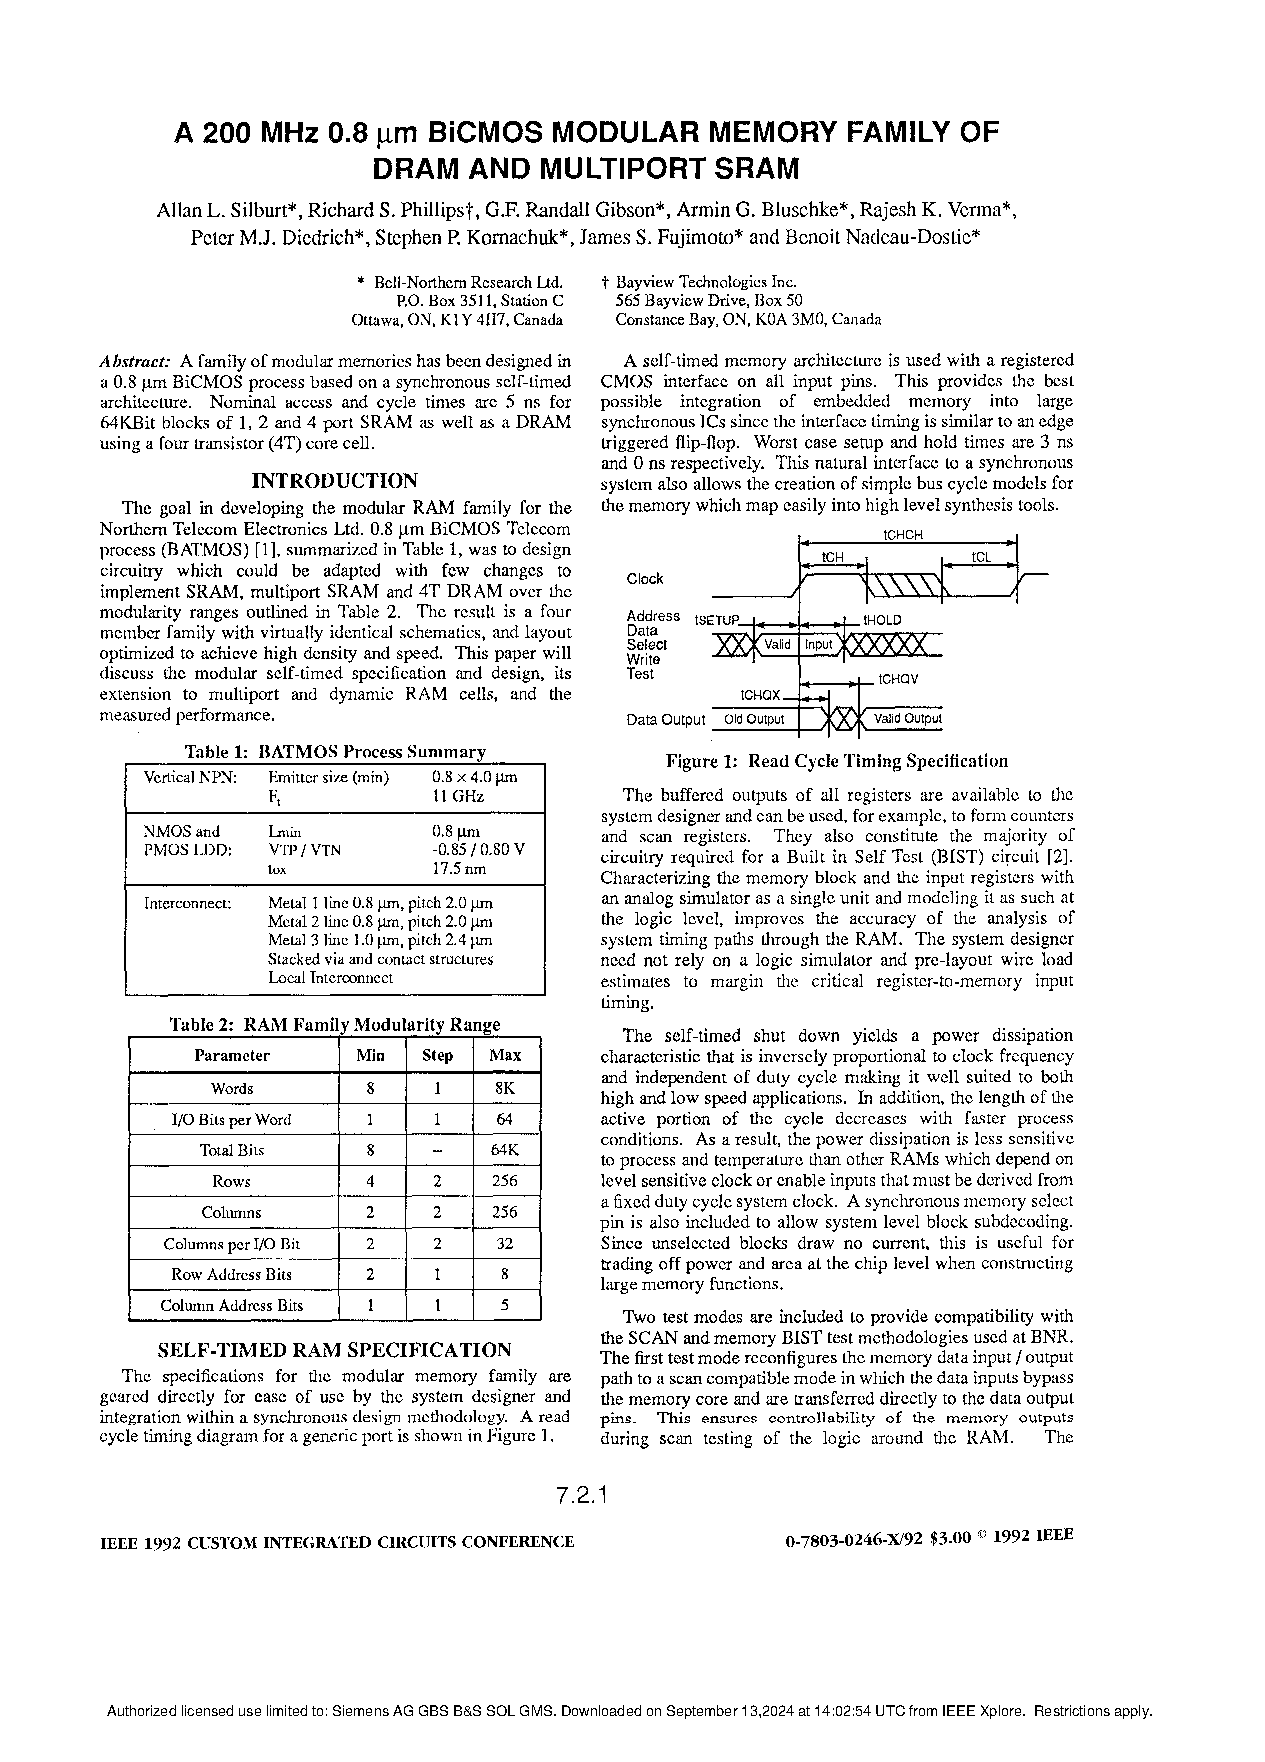
\includegraphics[height=\pdfheight]{Articles/publications/A_200_Mhz_0.8-spl_mu-m_BiCMOS_Modular_Memory_Family_Of_DRAM_And_Multiport_SRAM-page1.pdf}}
		}

%	\column{0.1}
%	\block[linewidth=\blw]{}{
%		\begin{tikzfigure}[]
%			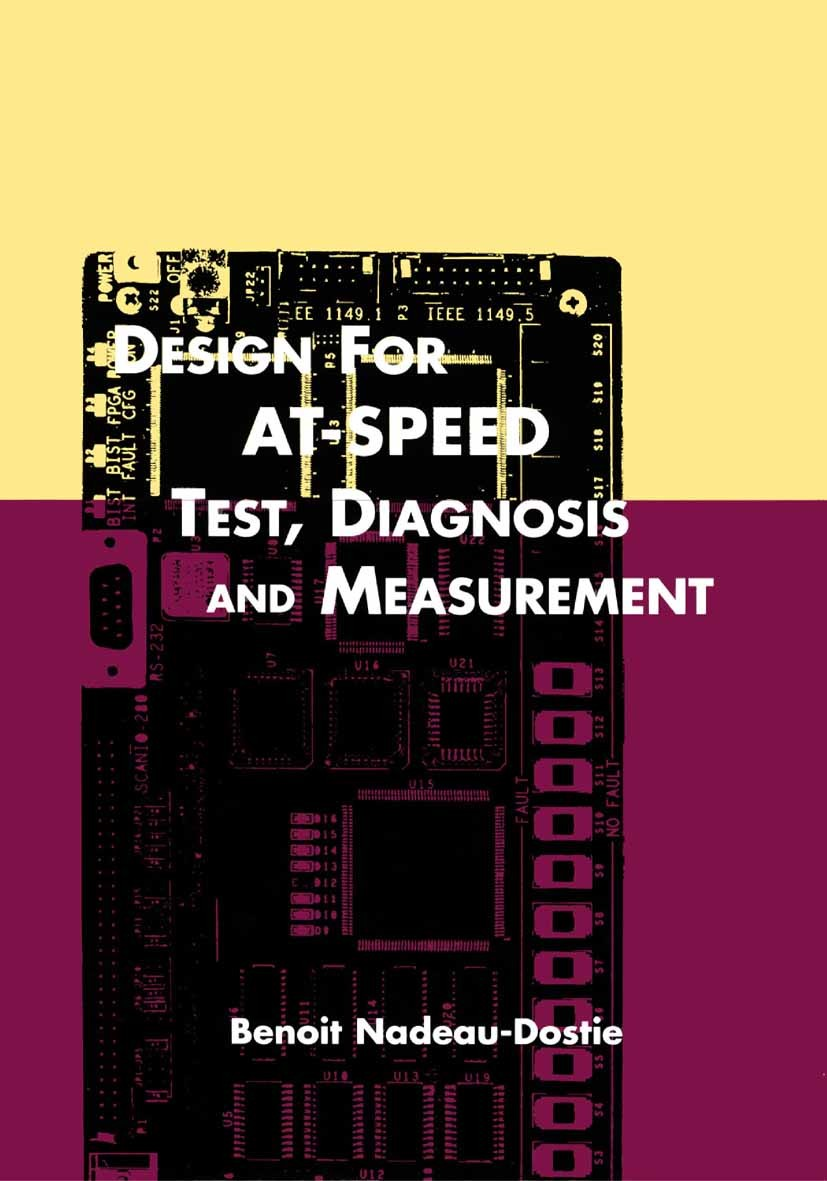
\includegraphics[width=\linewidth]{images/BND_Book}
%		\end{tikzfigure}
	}
	
	\column{0.5}
	
	\block[linewidth=\blw]{Patents}{
		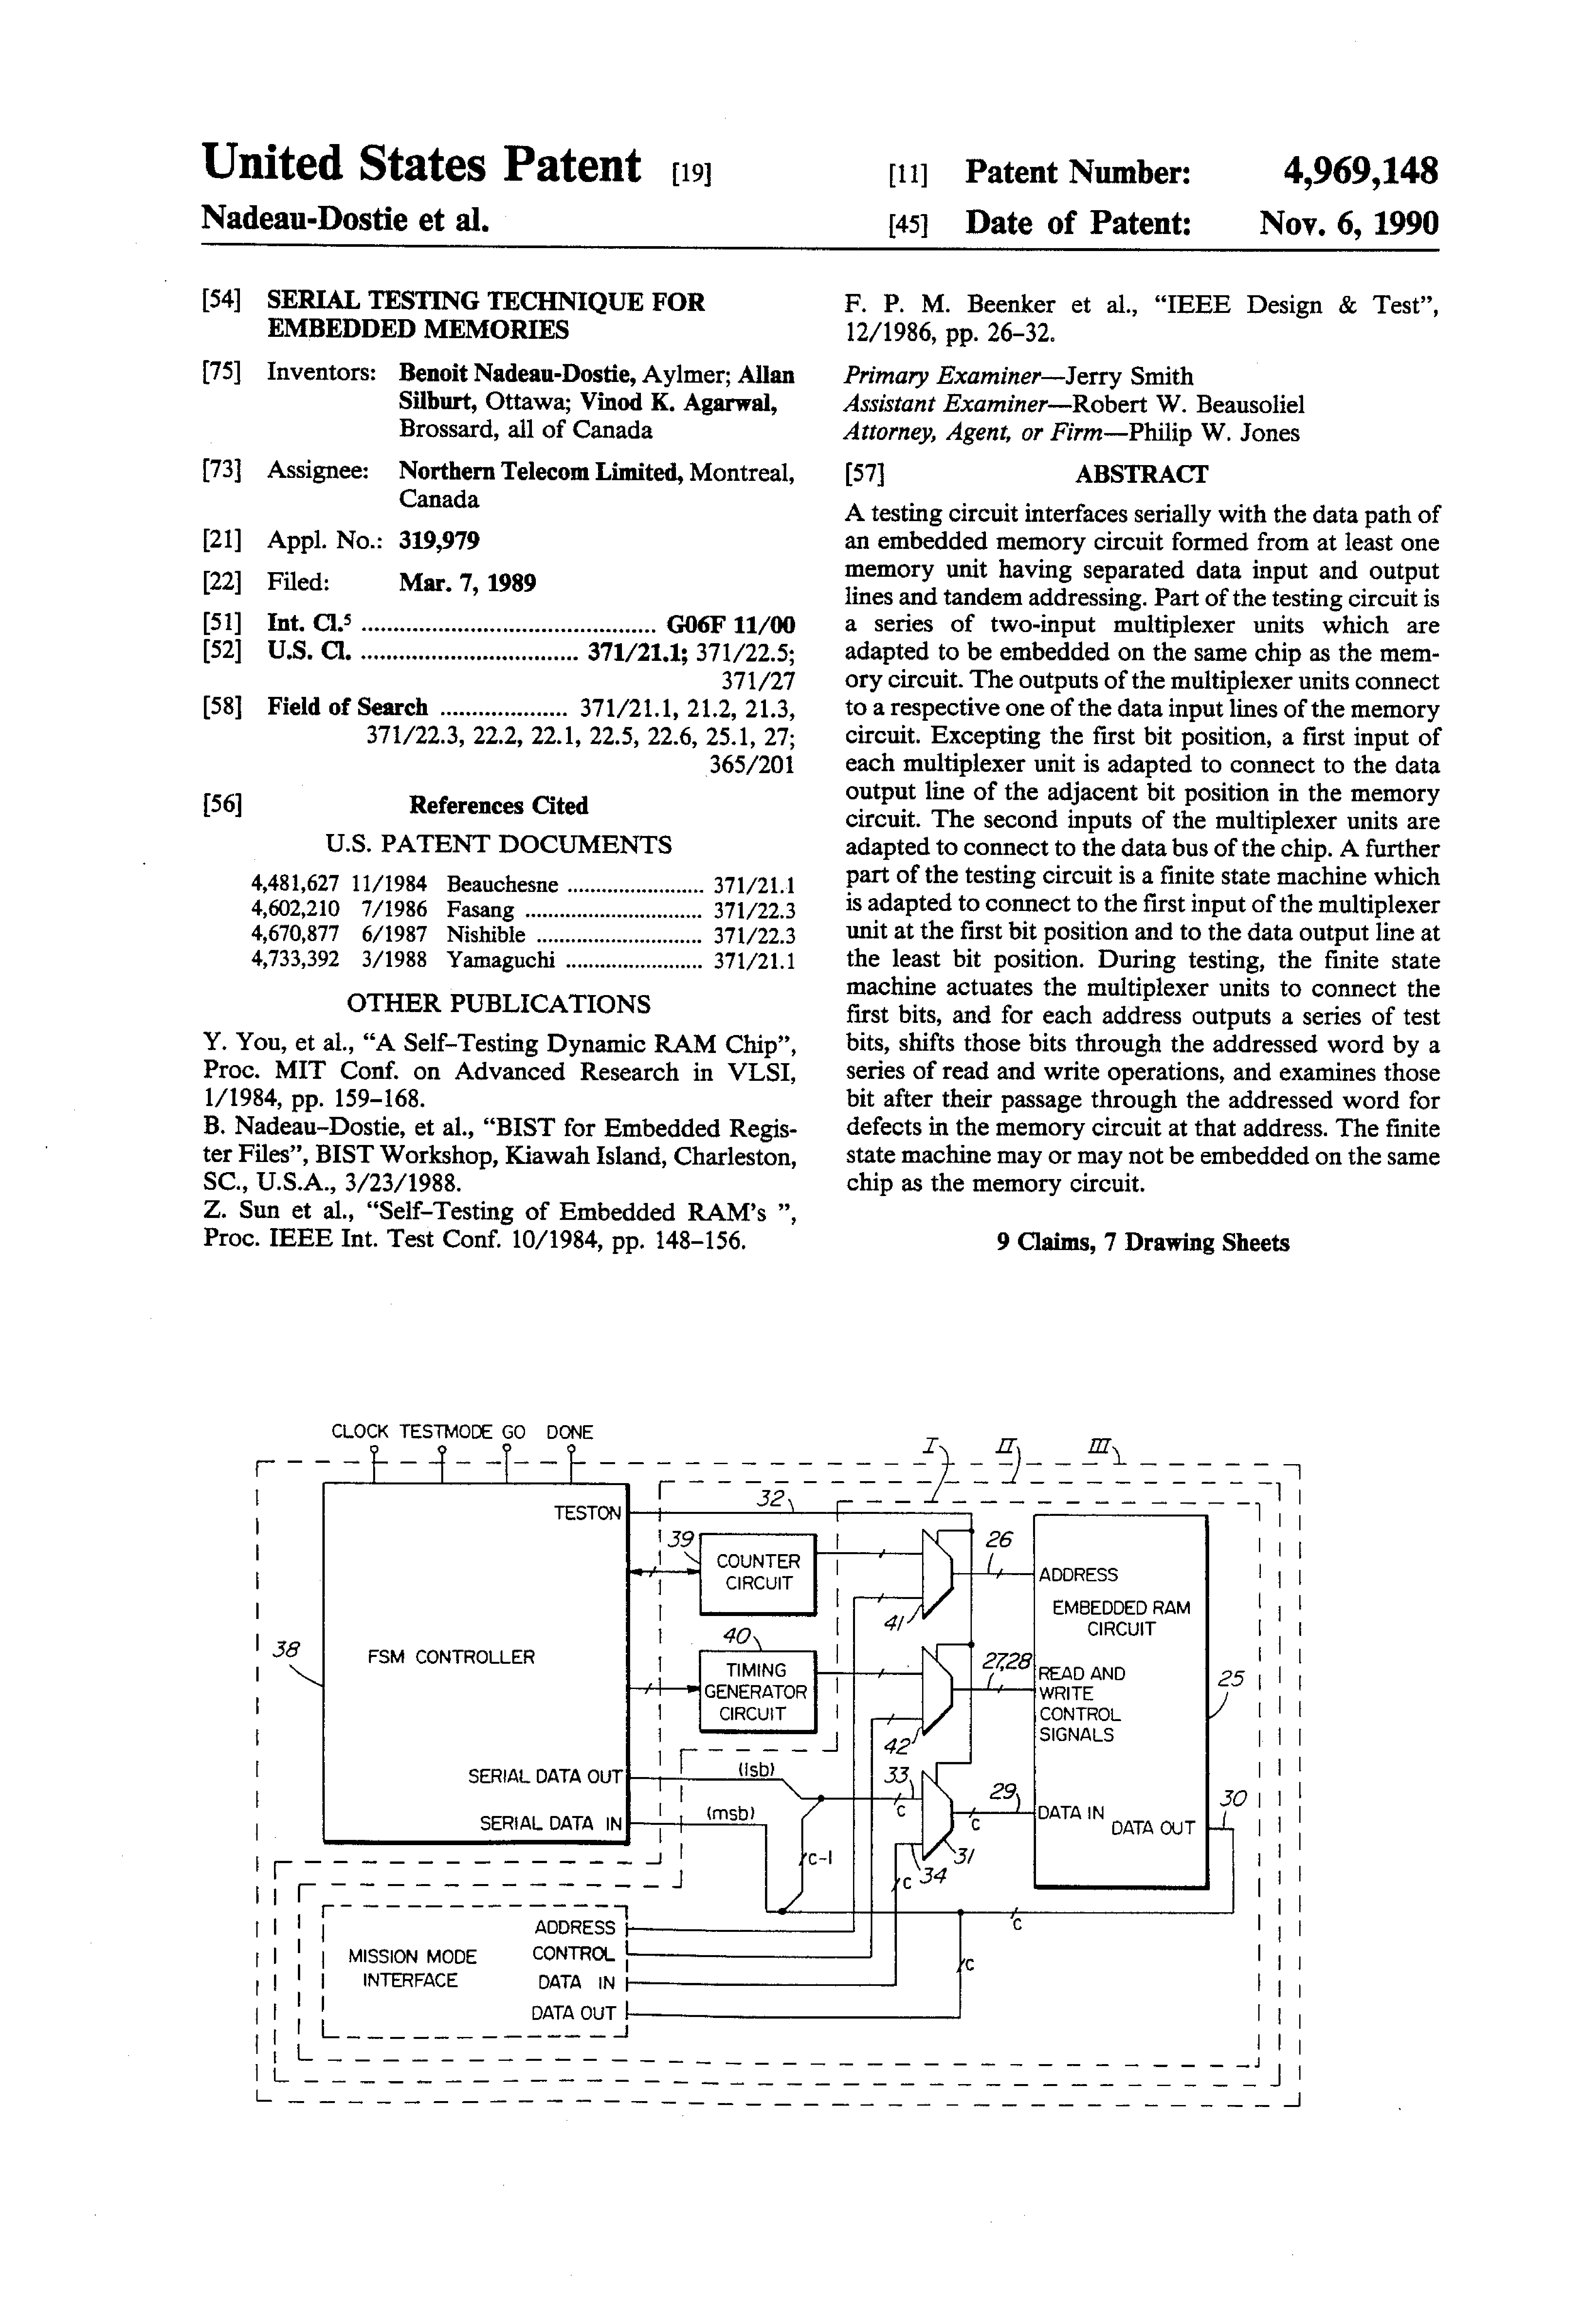
\includegraphics[width=\pdfwidth]{Patents/first_pages/1990_11_06_4969148-page1.pdf}
		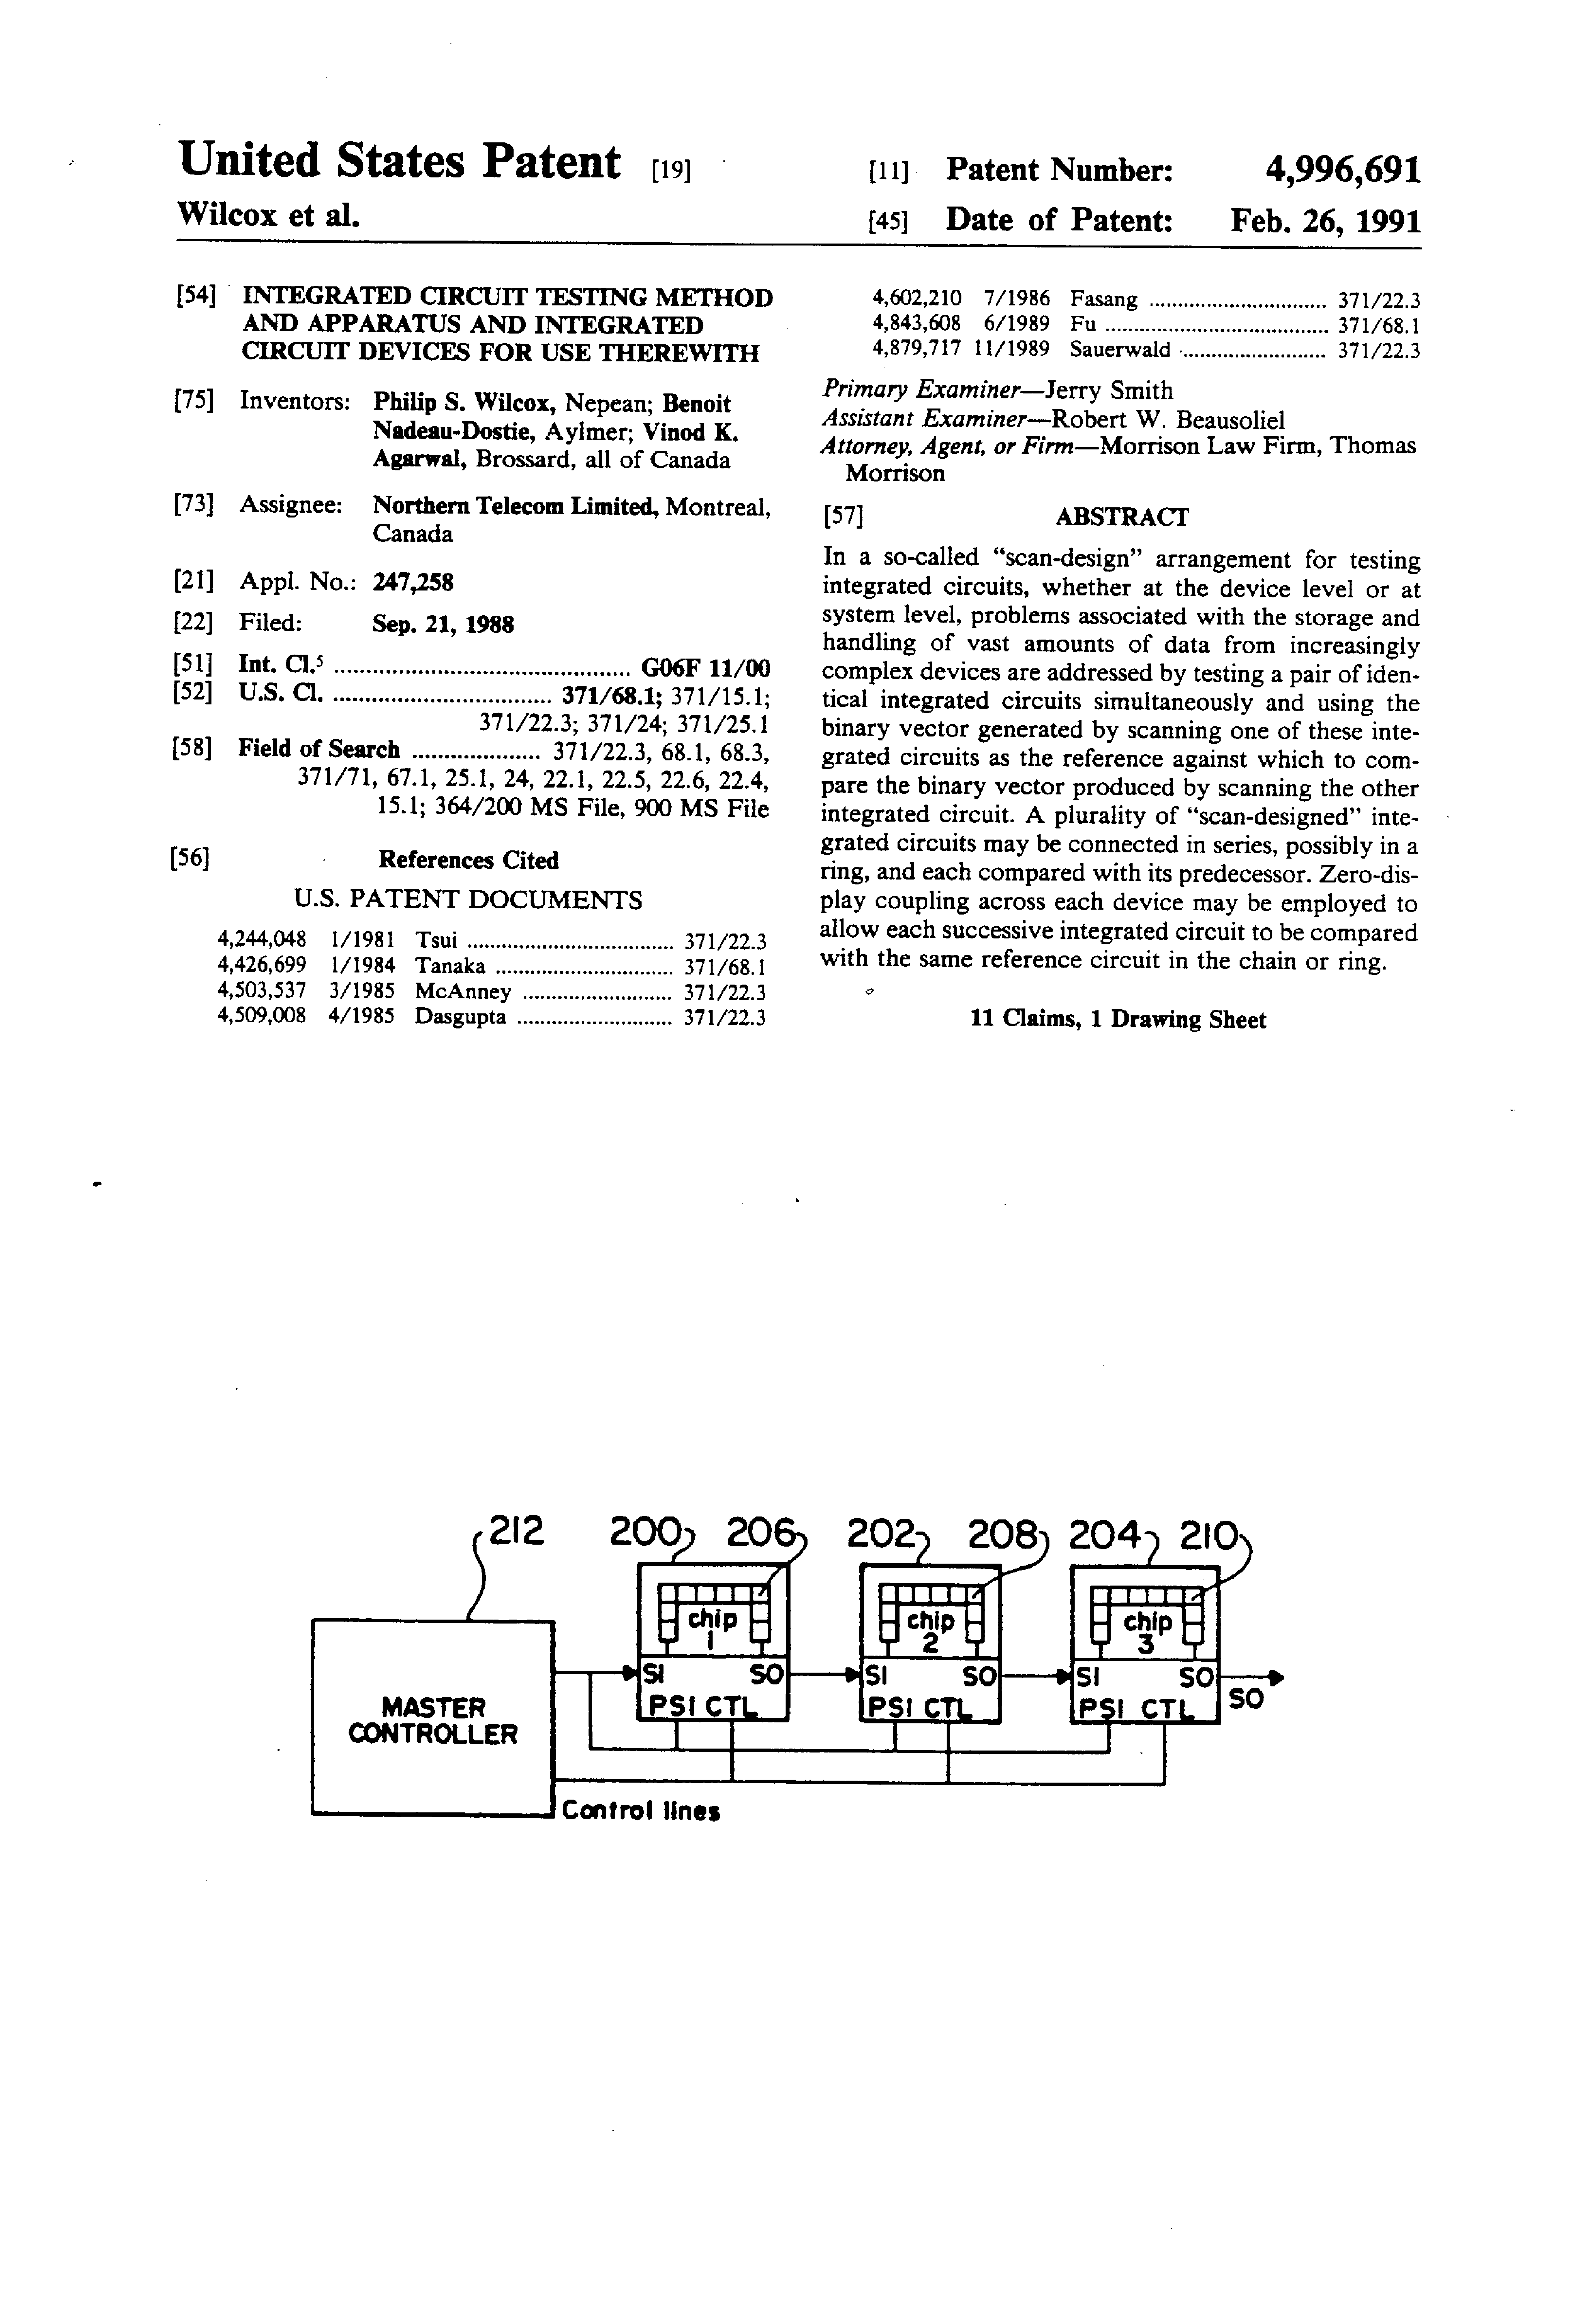
\includegraphics[width=\pdfwidth]{Patents/first_pages/1991_02_26_4996691-page1.pdf}
		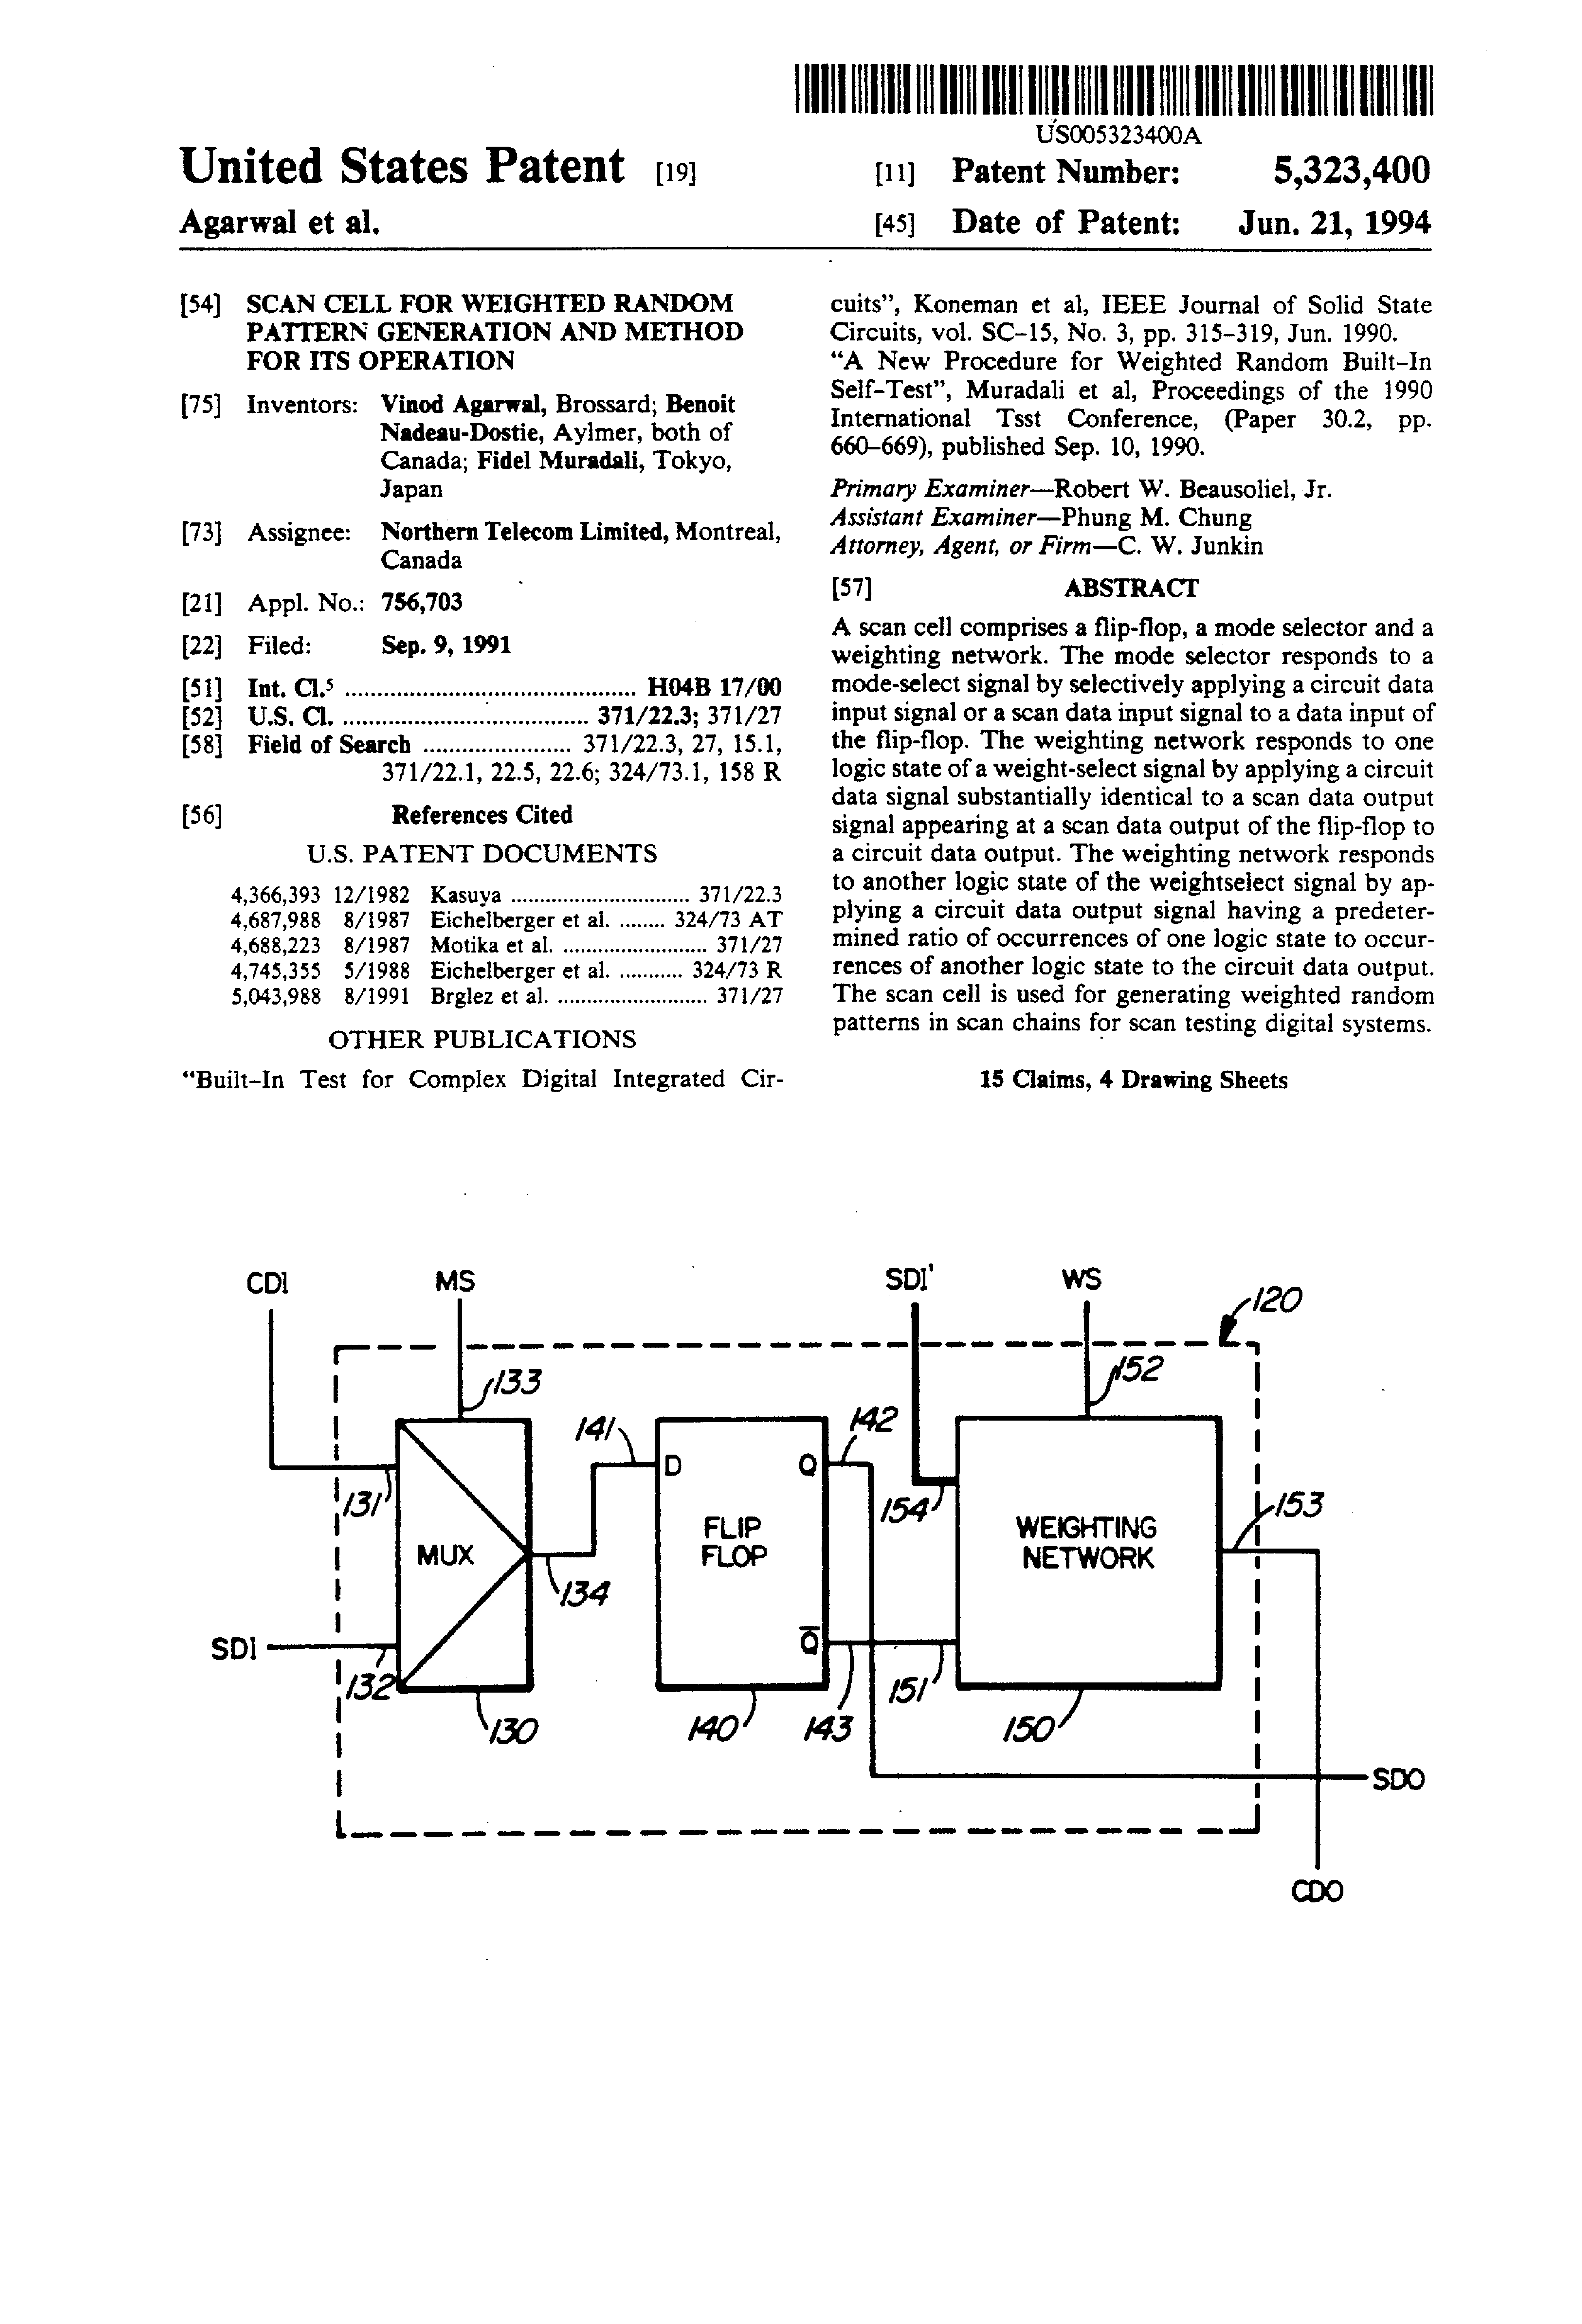
\includegraphics[width=\pdfwidth]{Patents/first_pages/1994_06_21_5323400-page1.pdf}
		
	}

\end{columns}


\end{document}